\documentclass{article}

\usepackage[portuguese]{babel}
\usepackage[utf8]{inputenc}
\usepackage[letterpaper,top=2cm,bottom=2cm,left=3cm,right=3cm,marginparwidth=1.75cm]{geometry}
\usepackage{amsmath}
\usepackage{graphicx}
\usepackage[colorlinks=true, allcolors=blue]{hyperref}
\usepackage{listings}
\usepackage{xcolor}
\usepackage{cite}
\usepackage{float}
\usepackage{lipsum}
\usepackage{tabularx}
\usepackage{pdflscape}
\usepackage{setspace}

\setstretch{1.5}
\lstset{
  language=Python,
  basicstyle=\ttfamily\small,
  numbers=left,
  numberstyle=\tiny\color{gray},
  keywordstyle=\color{blue},
  commentstyle=\color{gray},
  stringstyle=\color{orange},
  breaklines=true,
  frame=single,
  columns=flexible
}

\title{Avaliação 2 de Introdução a Computação}
\author{Nathan Loose Kuipper \\ \small{\texttt{251708041 | C3007834 | nathankuipper@gmail.com}} \\ Rafael Gontijo Ferreira \\ \small{\texttt{251708034 | C3007825 | rafael.gontijof2006@gmail.com}} }

\begin{document}
\maketitle

\begin{abstract}
Este trabalho analisa dados de sessões de cinema no Brasil usando Python e as bibliotecas \texttt{pandas}, \texttt{matplotlib} e \texttt{seaborn}. Quanto aos entregáveis, foram desenvolvidas respostas para cinco questões propostas juntamente a produção de tabelas e gráficos que trazem novos \textit{insights} acerca da base de dados. Essas análises incluem o cálculo de métricas como público total, média do público, desvio do público médio, tempo útil de exibição, distribuição geográfica das sessões, entre outras. As visualizações buscam destacar padrões como a concentração regional do público, variações no tempo de exibição entre países e diferenças entre filmes brasileiros e estrangeiros. O código-fonte, com versionamento ativo, está disponível no GitHub: \url{https://github.com/Gontijo8199/A2-IntroComp/tree/main}.
\end{abstract}
\pagebreak
\section{Introdução}
Este trabalho tem como objetivo analisar os dados contidos no arquivo \texttt{bilheteria.db}, referentes a sessões de cinema realizadas em diversos complexos no país. A partir dessas informações, foram respondidas as questões propostas, com a realização de agrupamentos e a geração de visualizações que fornecem \textit{insights} sobre a exibição e o consumo de filmes no Brasil. Utilizando a linguagem \texttt{Python} e bibliotecas como \texttt{pandas}, \texttt{matplotlib} e \texttt{seaborn}, foi feita a limpeza e análise dos dados, além da construção de tabelas e gráficos que facilitam a compreensão do cenário cinematográfico nacional.

\section{Análise exploratória dos dados}

O arquivo \texttt{bilheteria.db} contém sete tabelas utilizadas como base de dados para a realização deste trabalho:

\begin{itemize}
    \item \texttt{sessao}: Possui 1.748.362 linhas e as colunas \texttt{id}, \texttt{filme\_id}, \texttt{sala\_id}, \texttt{publico} e \texttt{data\_exibição}, servindo para obter dados sobre as sessões de cinema.

    \item \texttt{sala}: Possui 3.230 linhas e as colunas \texttt{id}, \texttt{nome} e \texttt{from\_complexo}, permitindo o acesso às informações sobre as salas de cinema.

    \item \texttt{complexo}: Possui 682 linhas e as colunas \texttt{id}, \texttt{municipio}, \texttt{UF} e \texttt{from\_exibidor}, contendo os dados sobre os municípios onde os filmes foram exibidos.

    \item \texttt{exibidor}: Possui 179 linhas e as colunas \texttt{id} e \texttt{from\_grupo}, relacionadas aos exibidores responsáveis pelos complexos.

    \item \texttt{distribuidora}: Possui 71 linhas e as colunas \texttt{id}, \texttt{nome} e \texttt{cnpj}, permitindo identificar as distribuidoras responsáveis por cada filme.

    \item \texttt{grupo\_exibidor}: Possui 63 linhas e apenas a coluna \texttt{id}, representando os grupos aos quais os exibidores pertencem.

    \item \texttt{filme}: Possui 514 linhas e as colunas \texttt{id}, \texttt{titulo\_original}, \texttt{titulo\_br}, \texttt{cpb\_roe}, \texttt{pais\_origem} e \texttt{from\_distribuidora}, contendo informações detalhadas sobre cada filme exibido.
\end{itemize}
\pagebreak
\subsection{Análise do Código e das Questões da Parte 1}
Nesta subseção, cada aspecto que compõe a Parte 1 do trabalho será analisado de forma minuciosa, ou seja, as cinco questões propostas e os módulos de apoio apresentados.
\subsection*{Módulo Auxiliar A2}
O Modulo \texttt{ModuloA2.py} foi importado em ambos arquivos \texttt{a2\_parte1.py} e \texttt{a2\_parte2.py}.

Além das funções \texttt{carrega\_tabela} e \texttt{lista\_tabelas}, foi implementada a função \texttt{queryconn}, que recebe como parâmetros o caminho da base de dados e uma consulta SQL. Utiliza o gerenciador de contexto \texttt{with} para abrir uma conexão temporária com o banco, garantindo o fechamento automático dos recursos após a execução.

Dentro da função, é criado um \texttt{cursor}, que permite executar comandos SQL diretamente no banco de dados. O método \texttt{fetchall()} é usado para recuperar todas as linhas resultantes da execução da consulta. A consulta propriamente dita é executada pela função \texttt{read\_sql\_query()}\footnote{A função \texttt{read\_sql\_query()} da biblioteca \texttt{pandas} executa uma consulta SQL em uma conexão de banco de dados e retorna os resultados em um \texttt{DataFrame}, facilitando a manipulação dos dados em Python.}, que retorna os dados diretamente em um \texttt{DataFrame}.


\linespread{1}
\begin{lstlisting}
AUTORES = ['Nathan Loose Kuipper', 'Rafael Gontijo Ferreira']

import pandas as pd 
import sqlite3
from pathlib import Path

PATH =  Path(__file__).parent # bilheteria.db na mesma pasta que esse arquivo

def queryconn(database, query):    
def queryconn(database, query):    
    with sqlite3.connect(database) as conn:
        cursor = conn.cursor()
        # cursor.execute("SELECT name FROM sqlite_master WHERE type='table';")
        # tables = cursor.fetchall() 
        # cursor.execute("SELECT name FROM sqlite_master WHERE type='table';")
        # tables = cursor.fetchall() 
        df = pd.read_sql_query(query, conn)


        return df
    
def carrega_tabela(database, tabela):

    ...

def lista_tabelas(db_filename):

   ...
    
if __name__ == '__main__':
    print("Importe esse modulo para auxilar com o manejo da base de dados!")
\end{lstlisting}
\pagebreak
\linespread{1.5}
\subsection*{Questão 1}
Na \textbf{Questão 1}, foi utilizado o método \texttt{sum()} para calcular a \textbf{bilheteria total}, somando todos os valores da coluna \texttt{publico} da tabela \texttt{sessao}. Essa coluna representa o número de espectadores em cada sessão registrada no banco de dados. Ao somar todos os valores dessa coluna, obtém-se o total acumulado de público de todos os filmes exibidos.

\linespread{1}
\begin{lstlisting}
def questao1(database):
    
    dados = PATH / database

    dsessao = a2.carrega_tabela(dados, 'sessao')
    total_bilheteria = dsessao['publico'].sum()

    return total_bilheteria

\end{lstlisting}
\linespread{1.5}
\subsection*{Questão 2}
Na \textbf{Questão 2}, novamente foi usado \texttt{groupby()} com \texttt{sum()} para calcular o público total por filme. O método \texttt{merge()}\footnote{No método \texttt{merge()}, o parâmetro \texttt{left\_on} especifica a coluna da tabela esquerda usada para junção, enquanto \texttt{right\_on} indica a coluna correspondente da tabela direita. O parâmetro \texttt{how} determina o tipo de junção: \texttt{'left'} mantém todas as linhas da tabela esquerda, incorporando as correspondências da direita; \texttt{'right'} faz o oposto; \texttt{'inner'} retorna apenas as linhas correspondentes em ambas; e \texttt{'outer'} retorna todas as linhas de ambas as tabelas, preenchendo com \texttt{NaN} onde não há correspondência.} integrou os dados das sessões com a tabela de filmes. O \texttt{fillna(0)} garantiu que filmes sem sessões tivessem público zero. A ordenação foi feita com \texttt{sort\_values()} e a seleção do maior foi realizada com \texttt{iloc[0]}.
\linespread{1}
\begin{lstlisting}
def questao2(database):

    dados = PATH / database

    dfilme = a2.carrega_tabela(dados, 'filme')
    dsessao = a2.carrega_tabela(dados, 'sessao')
def questao2(database):

    dados = PATH / database

    dfilme = a2.carrega_tabela(dados, 'filme')
    dsessao = a2.carrega_tabela(dados, 'sessao')
    dfsessao = dsessao.groupby(by=['filme_id'])['publico'].sum().reset_index()
    merged_df = dfilme.merge(dfsessao, left_on='id', right_on='filme_id', how='left')
    merged_df['publico'] = merged_df['publico'].fillna(0)
    
    paises = merged_df['pais_origem'].unique()
    
    
    dic = {}
    for pais in paises:        
    for pais in paises:        
        most_viewed_film = merged_df[merged_df['pais_origem'] == pais].sort_values(by='publico', ascending=False).iloc[0]
        dic[pais] = {
            'nome': dfilme.loc[dfilme['id'] == most_viewed_film['filme_id'], 'titulo_original'].item(),
            'publico': int(most_viewed_film['publico'])
        }
    return pd.DataFrame(dic) 
    return pd.DataFrame(dic) 
\end{lstlisting}

\linespread{1.5}
\pagebreak
\subsection*{Questão 3}
Na \textbf{Questão 3}, o método \texttt{merge()} foi usado para unir as tabelas \texttt{sessao}, \texttt{sala} e \texttt{complexo}. O agrupamento por cidade foi feito com \texttt{groupby()} seguido de \texttt{sum()}. O resultado foi ordenado de forma decrescente com \texttt{sort\_values()} e limitado às 100 primeiras linhas com \texttt{head(100)}.
\linespread{1}
\begin{lstlisting}
def questao3(database):

    dados = PATH / database
def questao3(database):

    dados = PATH / database
    
    dsessao = a2.carrega_tabela(dados, 'sessao')
    dsala = a2.carrega_tabela(dados, 'sala')[['id', 'from_complexo']]
    dcomplexo = a2.carrega_tabela(dados, 'complexo')[['id', 'municipio']]
    dsessao = a2.carrega_tabela(dados, 'sessao')
    dsala = a2.carrega_tabela(dados, 'sala')[['id', 'from_complexo']]
    dcomplexo = a2.carrega_tabela(dados, 'complexo')[['id', 'municipio']]

    df = dsessao.merge(dsala, left_on='sala_id', right_on='id', how='left')
    df = df.merge(dcomplexo, left_on='from_complexo', right_on='id', how='left')

    cidades = df.groupby('municipio', as_index=False)['publico'].sum()
    cidades = cidades.rename(columns={'publico': 'BILHETERIA'})

    top100 = cidades.sort_values('BILHETERIA', ascending=False).head(100).reset_index(drop=True)
    top100 = cidades.sort_values('BILHETERIA', ascending=False).head(100).reset_index(drop=True)

    return top100
\end{lstlisting}
\linespread{1.5}
\subsection*{Questão 4}
Na \textbf{Questão 4}, as tabelas foram integradas usando \texttt{merge()}. O método \texttt{rename()} foi aplicado para ajustar os nomes das colunas. O agrupamento por cidade e filme usou \texttt{groupby()} com \texttt{sum()}, seguido de uma ordenação com \texttt{sort\_values()} e seleção do filme de maior bilheteria em cada cidade usando \texttt{groupby().head(1)}.
\linespread{1}
\begin{lstlisting}
def questao4(database):

    dados = PATH / database
def questao4(database):

    dados = PATH / database
    
    dsessao = a2.carrega_tabela(dados, 'sessao')
    dsala = a2.carrega_tabela(dados, 'sala')[['id', 'from_complexo']]
    dcomplexo = a2.carrega_tabela(dados, 'complexo')[['id', 'municipio']]
    dfilme = a2.carrega_tabela(dados, 'filme')[['id', 'titulo_original']]
    dsessao = a2.carrega_tabela(dados, 'sessao')
    dsala = a2.carrega_tabela(dados, 'sala')[['id', 'from_complexo']]
    dcomplexo = a2.carrega_tabela(dados, 'complexo')[['id', 'municipio']]
    dfilme = a2.carrega_tabela(dados, 'filme')[['id', 'titulo_original']]

    df = dsessao.merge(dsala, left_on='sala_id', right_on='id', how='left')
    df = df.rename(columns={'id_x': 'sessao_id', 'id_y': 'sala_id'})  

    df = df.merge(dcomplexo, left_on='from_complexo', right_on='id', how='left')
    df = df.rename(columns={'municipio': 'CIDADE'})
    
    df = df.merge(dfilme, left_on='filme_id', right_on='id', how='left')
    df = df.rename(columns={'titulo_original': 'FILME'})

    bilheteria = df.groupby(['CIDADE', 'FILME'], as_index=False)['publico'].sum()
    bilheteria = bilheteria.rename(columns={'publico': 'BILHETERIA'})
    resultado = bilheteria.sort_values('BILHETERIA', ascending=False).groupby('CIDADE').head(1)

    return resultado[['CIDADE', 'FILME', 'BILHETERIA']].reset_index(drop=True)
    return resultado[['CIDADE', 'FILME', 'BILHETERIA']].reset_index(drop=True)

\end{lstlisting}

\subsection*{Questão 5}
\linespread{1.5}
Na \textbf{Questão 5}, foi criada a coluna \texttt{tipo} usando \texttt{apply()} e uma função auxiliar para classificar os filmes como BR ou ESTRANGEIRO. Em seguida, a bilheteria estrangeira foi calculada com \texttt{groupby()}, assim como a bilheteria total da cidade. As informações foram unidas com \texttt{merge()} e os valores ausentes tratados com \texttt{fillna(0)}, resultando nas colunas \texttt{CIDADE}, \texttt{BILHETERIA\_BR} e \texttt{BILHETERIA\_ESTRANGEIRA}.
Na \textbf{Questão 5}, foi criada a coluna \texttt{tipo} usando \texttt{apply()} e uma função auxiliar para classificar os filmes como BR ou ESTRANGEIRO. Em seguida, a bilheteria estrangeira foi calculada com \texttt{groupby()}, assim como a bilheteria total da cidade. As informações foram unidas com \texttt{merge()} e os valores ausentes tratados com \texttt{fillna(0)}, resultando nas colunas \texttt{CIDADE}, \texttt{BILHETERIA\_BR} e \texttt{BILHETERIA\_ESTRANGEIRA}.
\linespread{1}
\begin{lstlisting}
def questao5(database):
    dados = PATH / database

    dsessao = a2.carrega_tabela(dados, 'sessao')
    dsala = a2.carrega_tabela(dados, 'sala')[['id', 'from_complexo']]
    dcomplexo = a2.carrega_tabela(dados, 'complexo')[['id', 'municipio']]
    dfilme = a2.carrega_tabela(dados, 'filme')[['id', 'pais_origem']]
def questao5(database):
    dados = PATH / database

    dsessao = a2.carrega_tabela(dados, 'sessao')
    dsala = a2.carrega_tabela(dados, 'sala')[['id', 'from_complexo']]
    dcomplexo = a2.carrega_tabela(dados, 'complexo')[['id', 'municipio']]
    dfilme = a2.carrega_tabela(dados, 'filme')[['id', 'pais_origem']]

    df = dsessao.merge(dsala, left_on='sala_id', right_on='id', how='left')
    df = df.rename(columns={'id_x': 'sessao_id', 'id_y': 'sala_id'})

    df = df.merge(dcomplexo, left_on='from_complexo', right_on='id', how='left')
    df = df.rename(columns={'municipio': 'CIDADE'})
    df = df.merge(dfilme, left_on='filme_id', right_on='id', how='left')

    # Classificar tipo de filme
    def classificar_tipo(pais):
        if isinstance(pais, str):
            paises = [p.strip().upper() for p in pais.split(',')]
            if len(paises) == 1 and paises[0] == 'BRASIL':
                return 'BR'
        return 'ESTRANGEIRO'

    df['tipo'] = df['pais_origem'].apply(classificar_tipo)
    # Classificar tipo de filme
    def classificar_tipo(pais):
        if isinstance(pais, str):
            paises = [p.strip().upper() for p in pais.split(',')]
            if len(paises) == 1 and paises[0] == 'BRASIL':
                return 'BR'
        return 'ESTRANGEIRO'

    df['tipo'] = df['pais_origem'].apply(classificar_tipo)

    bilheteria_estrangeira = (
        df[df['tipo'] == 'ESTRANGEIRO']
        .groupby('CIDADE', as_index=False)['publico']
        .sum()
        .rename(columns={'publico': 'BILHETERIA_ESTRANGEIRA'})
    )
    bilheteria_total = (
        df.groupby('CIDADE', as_index=False)['publico']
        .sum()
        .rename(columns={'publico': 'BILHETERIA_BR'})
    )
    resultado = bilheteria_total.merge(
        bilheteria_estrangeira, on='CIDADE', how='left'
    ).fillna(0)

    resultado['BILHETERIA_ESTRANGEIRA'] = resultado['BILHETERIA_ESTRANGEIRA'].astype(int)
    resultado['BILHETERIA_BR'] = resultado['BILHETERIA_BR'].astype(int)
    resultado = resultado.sort_values(by='BILHETERIA_BR', ascending=False).reset_index(drop=True)

    return resultado
    bilheteria_estrangeira = (
        df[df['tipo'] == 'ESTRANGEIRO']
        .groupby('CIDADE', as_index=False)['publico']
        .sum()
        .rename(columns={'publico': 'BILHETERIA_ESTRANGEIRA'})
    )
    bilheteria_total = (
        df.groupby('CIDADE', as_index=False)['publico']
        .sum()
        .rename(columns={'publico': 'BILHETERIA_BR'})
    )
    resultado = bilheteria_total.merge(
        bilheteria_estrangeira, on='CIDADE', how='left'
    ).fillna(0)

    resultado['BILHETERIA_ESTRANGEIRA'] = resultado['BILHETERIA_ESTRANGEIRA'].astype(int)
    resultado['BILHETERIA_BR'] = resultado['BILHETERIA_BR'].astype(int)
    resultado = resultado.sort_values(by='BILHETERIA_BR', ascending=False).reset_index(drop=True)

    return resultado

\end{lstlisting}

\pagebreak
\linespread{1.5}
\section{Análise estatística descritiva dos dados}
\subsection*{Visualização 1:}
\begin{figure}[H]
    \centerline{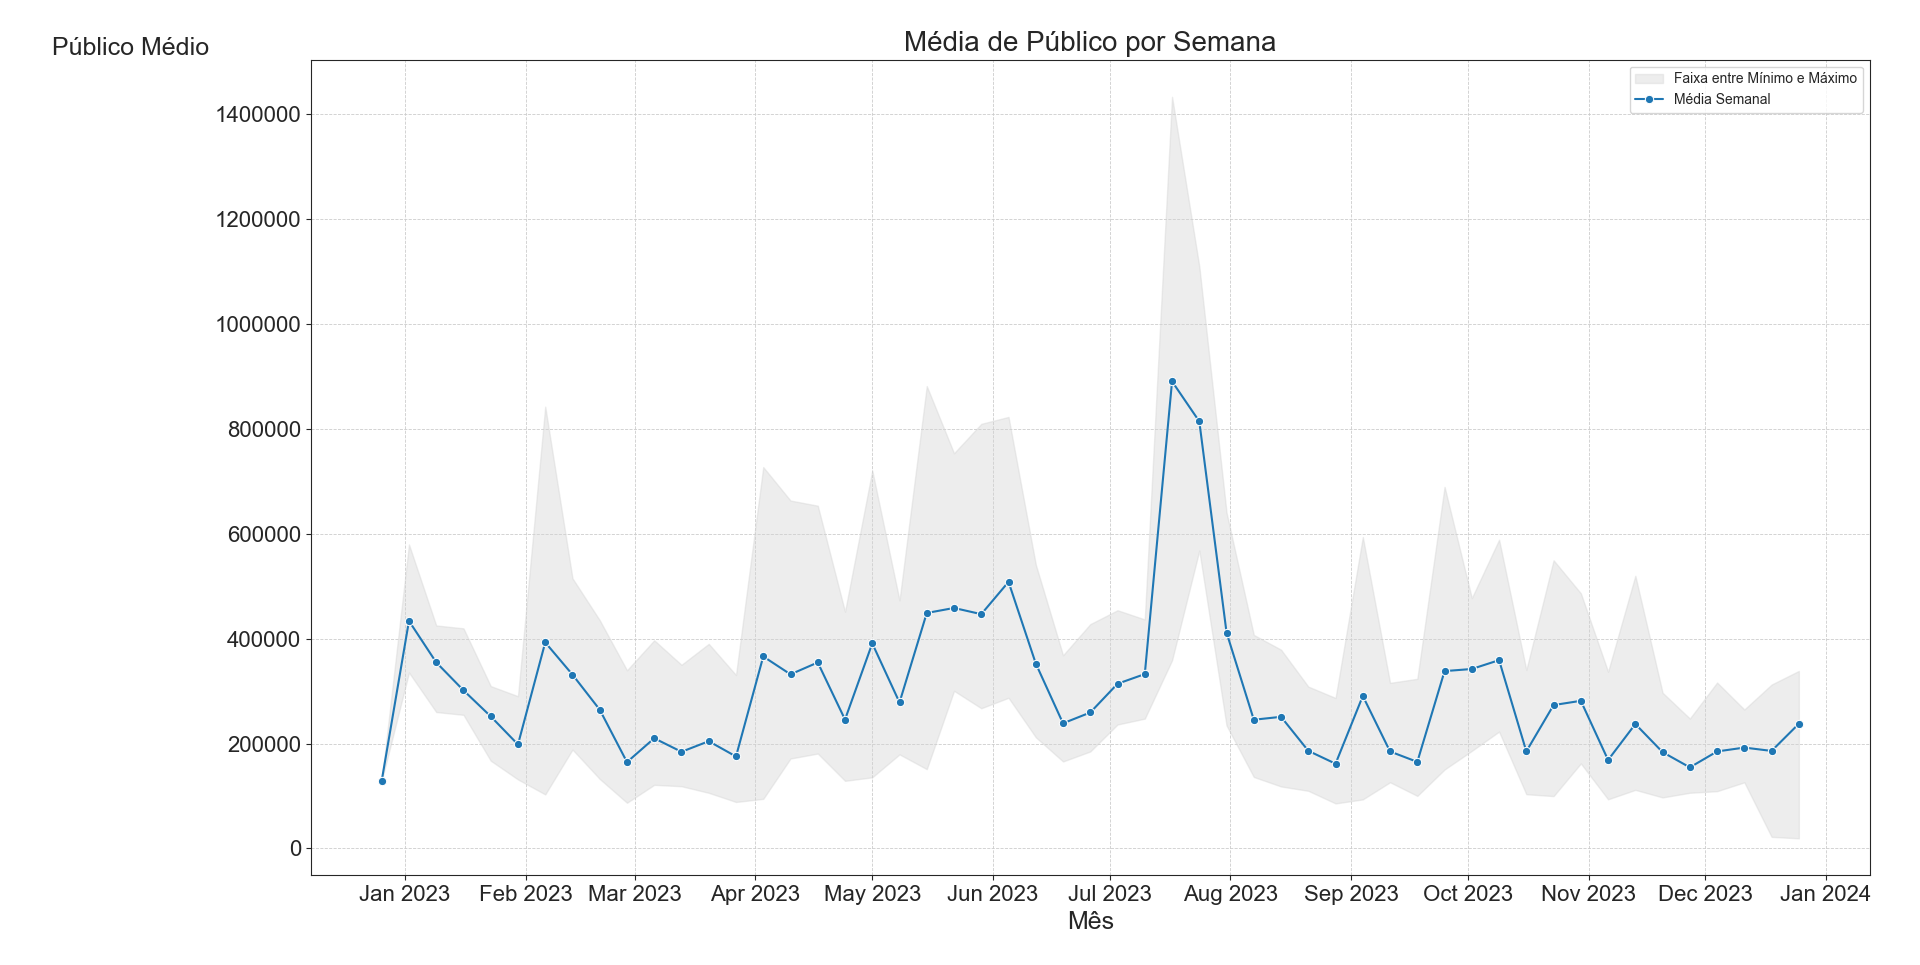
\includegraphics[width =\linewidth]{img/Figure_1.png}}
\end{figure}
A visualização apresenta a variação semanal da média de público ao longo de 2023, com dados diários agregados por data de exibição e convertidos para o tipo \texttt{datetime}. As datas foram transformadas em períodos semanais usando \texttt{dt.to\_period('W')} e uma função \texttt{lambda} para extrair o início da semana, permitindo o cálculo da média, mínimo e máximo de público semanal.

No gráfico, a faixa sombreada criada com \texttt{fill\_between} destaca a variação entre os valores mínimo e máximo, enquanto a linha com marcadores mostra a média semanal. Observa-se grande variação na audiência ao longo do ano, com picos em datas estratégicas, possivelmente relacionados a estreias de filmes e feriados, como o aumento notável registrado em julho. Ajustes no formato do eixo temporal e no estilo visual reforçam a clareza e facilitam a interpretação dos dados.


\subsection*{Visualização 2:}
\begin{figure}[H]
    \centerline{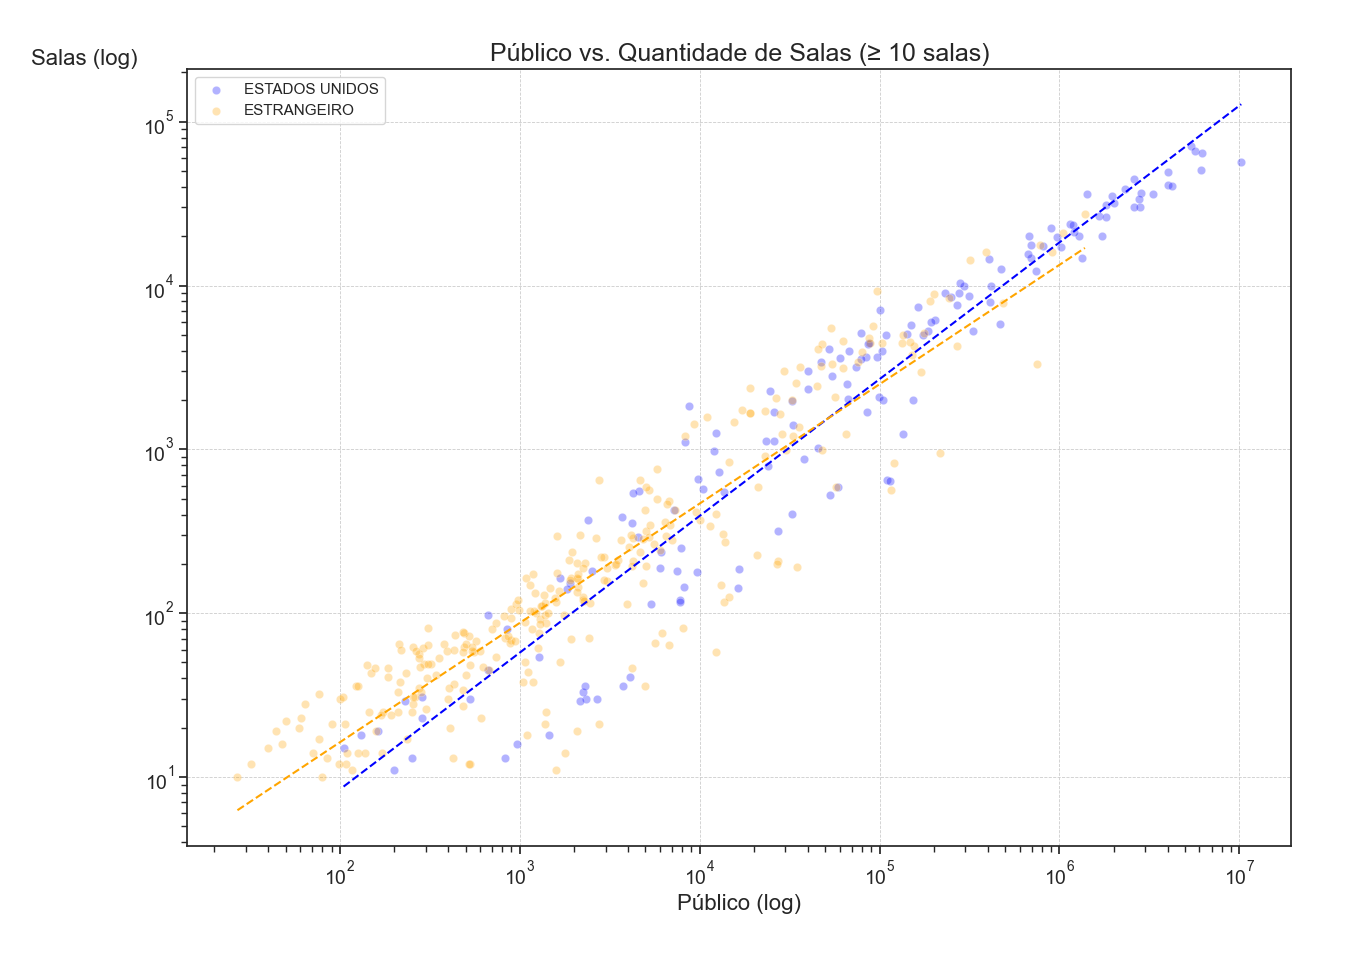
\includegraphics[width = \linewidth]{img/Figure_2.png}}
\end{figure}

A visualização relaciona o número de salas em que um filme foi exibido ao seu público total, considerando apenas filmes exibidos em 10 ou mais salas. Observa-se que quanto maior a quantidade de salas, maior tende a ser o público. A linha de regressão referente aos filmes americanos é mais acentuada que a dos demais grupos, indicando que o público cresce mais rapidamente com o número de salas para esses filmes. Além disso, essa reta atinge faixas de público entre \(10^{6}\) e \(10^{7}\), enquanto os demais permanecem abaixo desse intervalo.

O modelo de regressão linear no espaço logarítmico é dado por:

\[
\log_{10}(y) = a \cdot \log_{10}(x) + b
\]

onde \(y\) é a quantidade de salas, \(x\) o público, \(a\) a inclinação e \(b\) o intercepto da reta. No espaço original, a relação é:

\[
y = 10^{b} \cdot x^{a}
\]

Os parâmetros são estimados minimizando o erro quadrático:

\[
\min_{a,b} \sum_{i} \left( \log_{10}(y_i) - (a \cdot \log_{10}(x_i) + b) \right)^2
\]

com dados \(\{(x_i,y_i)\}\) positivos.

No código, os dados são agrupados por filme, somando público e salas, e filtrados para filmes exibidos em pelo menos 10 salas. As variáveis são transformadas em \(\log_{10}\) para linearizar a relação. Para cada grupo de país (Estados Unidos e estrangeiros), ajusta-se uma regressão linear via \texttt{statsmodels} \texttt{OLS}. O gráfico exibe pontos e linhas de regressão em escala log-log, com cores distintas, facilitando a visualização e destacando diferenças entre os grupos. A grade tracejada e fontes adequadas melhoram a legibilidade.

\subsection*{Visualização 3:}
\begin{figure}[H]
    \centerline{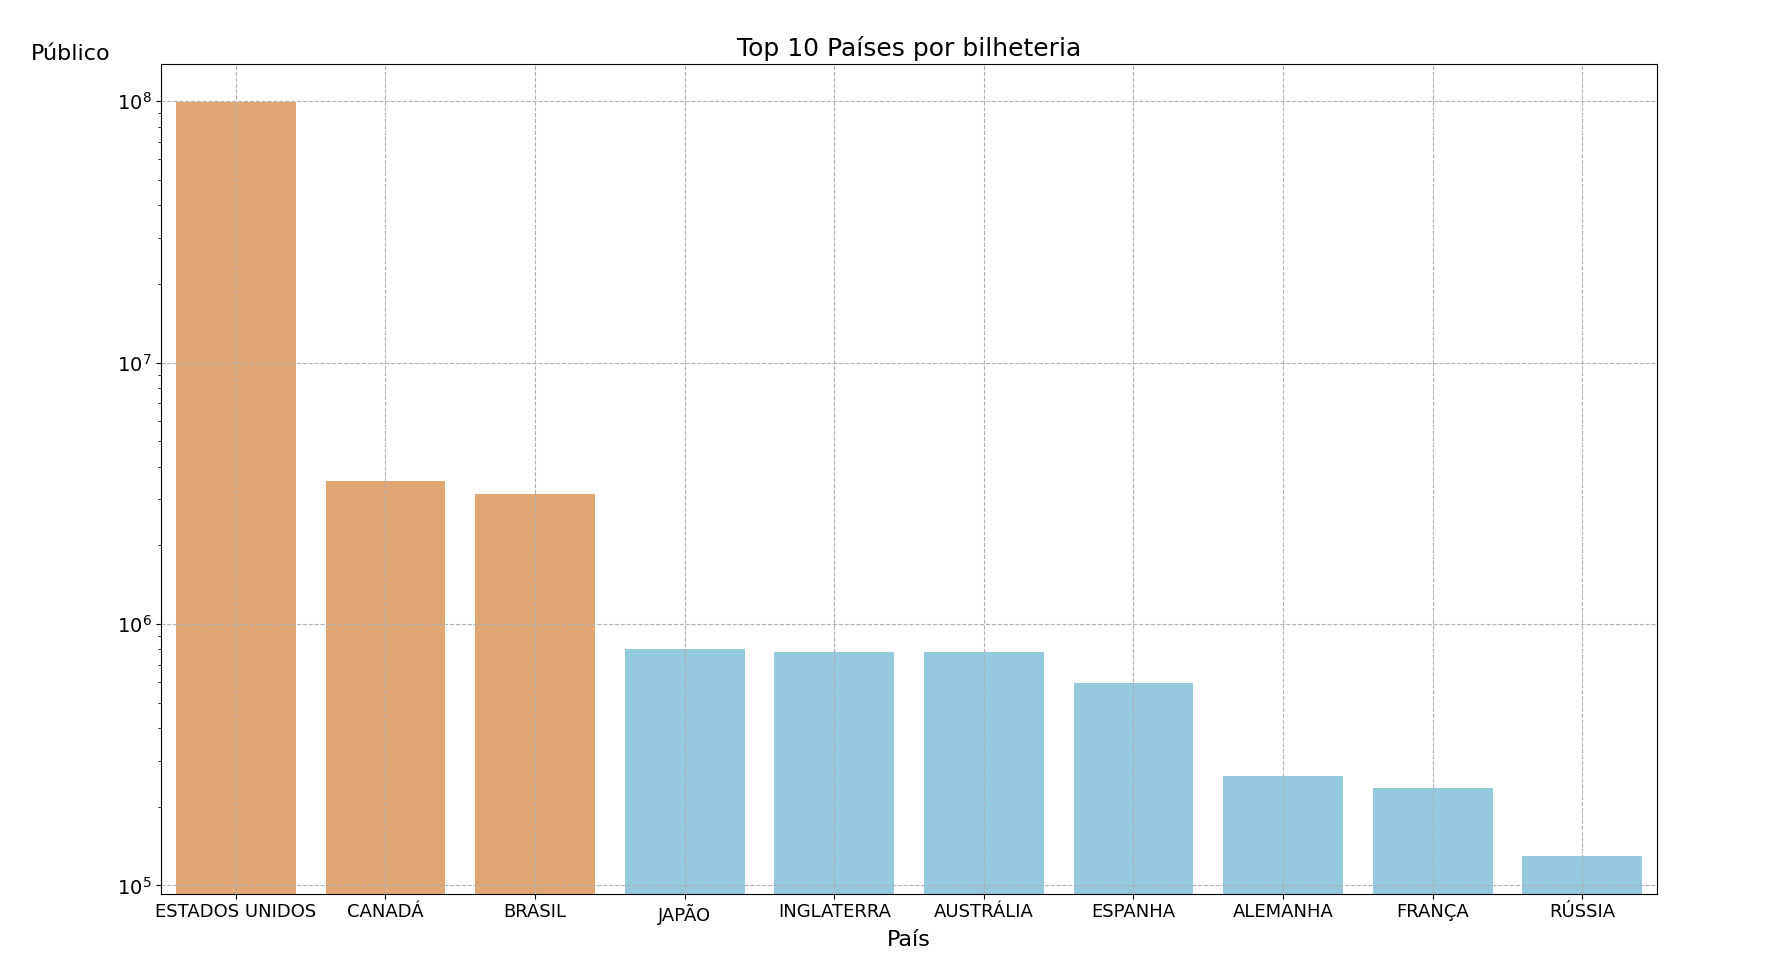
\includegraphics[width = \linewidth]{img/Figure_3.png}}
\end{figure}
A visualização foi dividida em dois gráficos de barras horizontais:

\begin{itemize}
    \item À esquerda, apresenta-se a bilheteria de filmes no cenário nacional por país de origem, destacando o Brasil com cor diferente para facilitar a identificação.
    \item À direita, apresenta-se a bilheteria de filmes brasileiros nas unidades da federação, com destaque para as três cidades com maior público, realçadas em cor distinta.
\end{itemize}

Essa diferenciação de cores tem o objetivo de garantir uma visualização clara e objetiva, facilitando a interpretação dos dados para o público-alvo.

\vspace{0.3cm}

No código, os dados são agrupados e somados para público e salas por filme, e então agrupados por país de origem para o gráfico global. No gráfico nacional, são filtradas as sessões de filmes brasileiros, somando o público por município e selecionando as dez cidades com maior bilheteria. A categorização das três principais cidades permite seu destaque visual.

O uso de \texttt{seaborn.barplot} facilita a criação das barras horizontais com as categorias destacadas. As anotações numéricas ao lado das barras indicam os valores exatos, melhorando a compreensão dos dados. A grade tracejada e a padronização das fontes garantem legibilidade e estética consistentes.


\subsection*{Visualização 4:}
\begin{figure}[H]
    \centerline{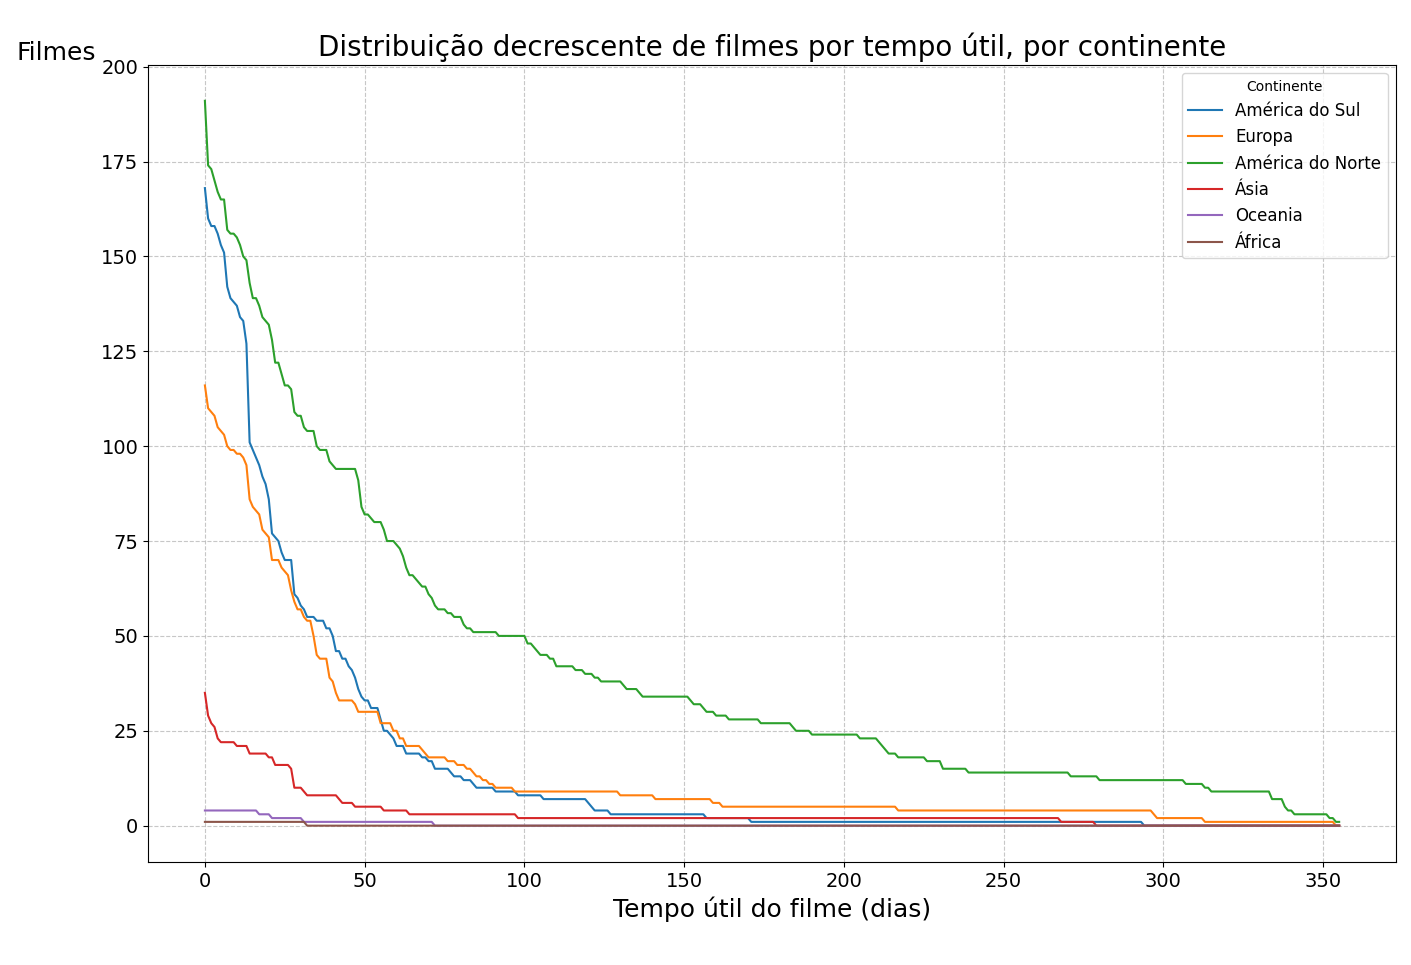
\includegraphics[width = \linewidth]{img/Figure_4.png}}
\end{figure}

O código realiza múltiplos \texttt{merge} entre as tabelas \texttt{sessao}, \texttt{filme}, \texttt{sala} e \texttt{complexo} para consolidar os dados necessários. A coluna \texttt{data\_exibicao} é convertida para o formato \texttt{datetime} para permitir o cálculo correto do intervalo entre a primeira e a última exibição de cada filme, definido como \texttt{tempo\_util\_dias}. Cada filme é associado a um continente por meio de um mapeamento manual baseado no país de origem.

A contagem decrescente de filmes exibidos por no mínimo determinado número de dias é calculada para cada continente, permitindo comparar a longevidade média dos filmes por região. A visualização evidencia que a América do Norte mantém filmes em exibição por períodos significativamente maiores, enquanto continentes como África e Oceania apresentam ciclos de exibição mais curtos.


\subsection*{Tabela 1}

\begin{table}[H]
\centering
\caption{Tempo útil médio de exibição por país de origem\\}
\begin{small}
\begin{tabular}{l r}
\hline
\textbf{País de Origem} & \textbf{Tempo Útil Médio (dias)} \\
\hline
SUÉCIA & 161.00 \\
CHINA & 143.75 \\
BELARUS (BIELORUSSIA) & 129.00 \\
ESPANHA & 109.60 \\
IRÃ & 97.00 \\
ESTADOS UNIDOS & 75.43 \\
CANADÁ & 75.22 \\
POLÔNIA & 73.60 \\
ÁUSTRIA & 68.00 \\
BÉLGICA & 58.00 \\
COLÔMBIA & 58.00 \\
ALEMANHA & 55.44 \\
EMIRADOS ÁRABES UNIDOS & 55.00 \\
PANAMÁ & 54.00 \\
HOLANDA & 41.00 \\
\end{tabular}
\end{small}

\begin{center}
\small
\ldots
\end{center}

\end{table}
A tabela apresenta o tempo útil médio de exibição dos filmes por país de origem, em dias, com base nos registros de sessões de cinema. O cálculo considerou a diferença entre a primeira e a última exibição de cada filme, obtida após a junção de tabelas com informações de filmes, salas e complexos. As datas foram tratadas com \texttt{pd.to\_datetime()} e, posteriormente, os tempos foram agregados por país, utilizando média aritmética.


 
A partir da análise da tabela pode-se notar que o tempo médio de exibição não segue estritamente o tamanho ou poder da indústria cinematográfica.
Isso porque, países menos centrais em termos de volume de produção podem ter filmes com maior longevidade. Enquanto grandes produtores,
como os EUA, mesmo com forte presença global, apresentam tempos mais moderados, possivelmente devido à maior rotatividade de lançamentos.

\pagebreak
\subsection*{Tabela 2}

\begin{table}[H]
\centering
\caption{Estatísticas de público por filme: média, desvio padrão, moda do dia da semana, semana do mês e mês de exibição\\}
\begin{small}
\begin{tabularx}{\textwidth}{X r r l c c}
\hline
\textbf{Título} & \textbf{Média Público} & \textbf{Desvio ($\sigma$)} & \textbf{Moda Dia} & \textbf{Moda Semana} & \textbf{Moda Mês} \\
\hline
FALE COMIGO & 227.83 & 299.91 & Quinta-feira & 3 & 8 \\
GODZILLA MINUS ONE & 227.07 & 216.66 & Quinta-feira & 2 & 12 \\
DECISÃO DE PARTIR & 211.83 & 231.45 & Quinta-feira & 2 & 1 \\
13 EXORCISMOS & 205.23 & 154.26 & Quinta-feira & 4 & 2 \\
BARBIE & 181.65 & 241.66 & Sábado & 4 & 8 \\
TRIÂNGULO DA TRISTEZA & 180.03 & 208.68 & Quinta-feira & 2 & 2 \\
THE CHOSEN... & 179.42 & 102.65 & Quinta-feira & 1 & 9 \\
TUDO EM TODO... & 169.97 & 197.06 & Quinta-feira & 3 & 3 \\
SAPATINHO VERMELHO... & 161.00 & --- & Quinta-feira & 3 & 4 \\
ENCANTO & 160.00 & --- & Quarta-feira & 2 & 12 \\

\end{tabularx}
\end{small}
\begin{center}
$\ldots$
\end{center}
\end{table}
A tabela apresenta um conjunto de estatísticas descritivas sobre o desempenho de público por filme, incluindo a média, o desvio padrão e a moda de três variáveis temporais: dia da semana, semana do mês e mês do ano. O cálculo foi realizado a partir da base de sessões, com junções das tabelas de filmes, salas e complexos para enriquecimento dos dados. As datas foram convertidas para o formato de data utilizando \texttt{pd.to\_datetime()}, e novas colunas categóricas foram derivadas para representar o dia da semana, o número da semana dentro do mês e o mês do ano. As funções de moda foram implementadas de forma personalizada para garantir o funcionamento em casos de ausência de valor ou outras exceções.

A análise destaca que o filme Fale Comigo obteve a maior média de público (227,83), mas também o maior desvio padrão (299,91), indicando alta variabilidade na ocupação das sessões. Além disso, observa-se um padrão de concentração de público nas quintas-feiras, sugerindo influência de estratégias de lançamento ou de programação das redes exibidoras.


\begin{landscape}
\subsection*{Tabela 3}
\begin{table}[H]
\centering
\small
\caption{Métricas de Exibição por Distribuidora\\}
\begin{tabular}{p{5cm}rrrrr}
\hline
\textbf{Distribuidora} & \textbf{Público} & \textbf{Total de Sessões} & \textbf{Média por Sessão} & \textbf{Desvio ($\sigma$)} & \textbf{Tempo Útil Médio (dias)} \\
\hline
WARNER BROS. (SOUTH) INC. & 52.935.246 & 688.130 & 76,93 & 116,40 & 96,24 \\
THE WALT DISNEY COMPANY (BRASIL) LTDA. & 24.273.591 & 341.583 & 71,06 & 89,57 & 83,76 \\
SM DISTRIBUIDORA DE FILMES LTDA & 9.547.406 & 195.485 & 48,84 & 70,37 & 30,52 \\
COLUMBIA TRISTAR FILMES DO BRASIL LTDA & 8.343.669 & 181.091 & 46,07 & 67,41 & 97,00 \\
PARAMOUNT PICTURES BRASIL DISTRIBUIDORA DE FILMES LTDA & 7.870.782 & 151.971 & 51,79 & 64,63 & 155,94 \\
DIAMOND FILMS DO BRASIL PRODUÇÃO E DISTRIBUIÇÃO DE FILMES LTDA & 1.993.412 & 22.267 & 89,52 & 161,46 & 36,24 \\
WMIX DISTRIBUIDORA LTDA. & 1.919.667 & 71.127 & 26,99 & 37,84 & 57,29 \\
VITRINE FILMES LTDA & 531.904 & 10.163 & 52,34 & 89,98 & 33,89 \\
ANTONIO FERNANDES FILMES LTDA & 444.162 & 9.968 & 44,56 & 56,83 & 46,80 \\
UNITED CINEMAS INTERNATIONAL BRASIL LTDA. & 357.937 & 8.165 & 43,84 & 60,57 & 9,80 \\
CINECOLOR DO BRASIL LTDA & 316.779 & 9.411 & 33,66 & 47,82 & 10,54 \\
FREESPIRIT DISTRIBUIDORA DE FILMES LTDA. & 225.561 & 11.002 & 20,50 & 27,08 & 40,25 \\
SA DISTRIBUIDORA DE CONTEÚDO AUDIOVISUAL LTDA & 216.849 & 955 & 227,07 & 216,66 & 27,00 \\
PLAYARTE PICTURES ENTRETENIMENTOS LTDA. & 191.989 & 10.282 & 18,67 & 23,70 & 25,40 \\
H2O DISTRIBUIDORA DE FILMES LTDA & 185.049 & 5.893 & 31,40 & 59,81 & 42,67 \\





\end{tabular}
\begin{center}
$\ldots$
\end{center}
\end{table}
\end{landscape}

Esta tabela reúne estatísticas que avaliam o desempenho das principais distribuidoras no mercado brasileiro, considerando volume total de público, número de sessões, média e desvio padrão do público por sessão, além do tempo útil médio de exibição dos filmes.

Tecnicamente, os dados foram consolidados por meio de múltiplas junções entre as tabelas de sessões, filmes, salas, complexos e distribuidoras. A conversão das datas permitiu calcular o tempo útil de cada filme pela diferença entre a primeira e última exibição. Em seguida, os indicadores foram agregados por distribuidora, possibilitando uma análise de alcance e duração de exibição, destacando a WARREN BROS. (SOUTH) INC como líder nos principais indicadores.


\section*{Conclusão}

Através deste trabalho, foi possível realizar uma análise abrangente sobre o desempenho da cinematografia ao redor do mundo, com ênfase em métricas de bilheteria, tempo de exibição, distribuição geográfica e estratégias de distribuidoras.

Por meio das visualizações e tabelas, destacam-se conclusões interessantes, como o protagonismo das quintas-feiras nas estreias e picos de público, alinhado às práticas tradicionais do setor cinematográfico. Além disso, é possivél notar que filmes com maior média de público, como Fale Comigo ou Godzilla Minus One, apresentam altos desvios, indicando grande variação na lotação das sessões.

Embora existam estados com maior concentração de público para filmes brasileiros, os dados evidenciam a hegemonia das produções norte-americanas em quase todos os aspectos de consumo, seja em alcance nacional, número de salas ou volume de público. 

\pagebreak
\begin{thebibliography}{99}

\bibitem{seaborn_examples}
Seaborn Development Team (2024). \textit{Seaborn Example Gallery}. Disponível em: \url{https://seaborn.pydata.org/examples/index.html}.

\bibitem{matplotlib_gallery}
Matplotlib Development Team (2024). \textit{Matplotlib Example Gallery}. Disponível em: \url{https://matplotlib.org/stable/gallery/index.html}.

\bibitem{matplotlib_colors}
Matplotlib Development Team (2024). \textit{Named Colors in Matplotlib}. Disponível em: \url{https://matplotlib.org/stable/gallery/color/named_colors.html}.

\bibitem{matplotlib_colormaps}
Matplotlib Development Team (2024). \textit{Colormaps in Matplotlib}. Disponível em: \url{https://matplotlib.org/stable/users/explain/colors/colormaps.html}.

\bibitem{tufte_visual_display}
Tufte, E. R. (2001). \textit{The Visual Display of Quantitative Information} (2ª ed.). Cheshire, CT: Graphics Press.

\bibitem{tufte_visual_explanations}
Tufte, E. R. (1997). \textit{Visual Explanations: Images and Quantities, Evidence and Narrative}. Cheshire, CT: Graphics Press.

\end{thebibliography}


\end{document}
